
\hwpart{IV}{Ablation Study (10 + 20 points)}
In this part of the homework, we will explore different design choices of the DDPM algorithm and how they can affect the final performance.

\question{Alternative Parametrization}{optional extra credits, 20}

\textcolor{cmured}{Note: By popular demand, this question is now an option extra credit question. I.e. You don't have to do it if you don't want to. The homework now have a total of 80 points instead of 100. If you still complete that question you will receive 20 points extra credit.}

\subq{a}{7} The original DDPM paper parametrized the model to predict the noise $\epsilon$. However, this is not the only option! First derive an alternative parametrization for the same model (i.e. what else can the model predict that can still yield the same mathematical formulation of the algorithm).

\answerbox{}{
The forward process can be written as
\[
x_t
=
\sqrt{\bar{\alpha}_t}x_0
+
\sqrt{1-\bar{\alpha}_t}\epsilon,
\qquad
\epsilon \sim \mathcal{N}(0,I).
\]
The original DDPM parameterization trains the network to predict
\(\epsilon\). This is convenient because once we have
\(\hat{\epsilon}_\theta(x_t,t)\), we can estimate
\[
\hat{x}_0
=
\frac{x_t-\sqrt{1-\bar{\alpha}_t}\hat{\epsilon}_\theta(x_t,t)}
{\sqrt{\bar{\alpha}_t}},
\]
and then use this estimate inside the reverse mean.

An equivalent alternative is to train the model to predict \(x_0\) directly:
\[
y_\theta(x_t,t)=\hat{x}_{0,\theta}(x_t,t),
\qquad
y=x_0.
\]
This still gives the same DDPM reverse formulation because the corresponding
noise prediction can be recovered by rearranging the forward-process equation:
\[
\hat{\epsilon}_\theta(x_t,t)
=
\frac{x_t-\sqrt{\bar{\alpha}_t}\hat{x}_{0,\theta}(x_t,t)}
{\sqrt{1-\bar{\alpha}_t}}.
\]

Another common alternative is the velocity parameterization
\[
v_t
=
\sqrt{\bar{\alpha}_t}\epsilon
-
\sqrt{1-\bar{\alpha}_t}x_0.
\]
If the network predicts \(\hat{v}_\theta(x_t,t)\), then both \(x_0\) and
\(\epsilon\) can be recovered by the linear inverse:
\[
\hat{x}_{0,\theta}
=
\sqrt{\bar{\alpha}_t}x_t
-
\sqrt{1-\bar{\alpha}_t}\hat{v}_\theta(x_t,t),
\]
\[
\hat{\epsilon}_\theta
=
\sqrt{1-\bar{\alpha}_t}x_t
+
\sqrt{\bar{\alpha}_t}\hat{v}_\theta(x_t,t).
\]
Thus, velocity prediction is only a different coordinate system for the same
two-dimensional linear relationship between \(x_0\), \(\epsilon\), and \(x_t\).

A more score-matching-flavored option is to predict the score of
\(q(x_t|x_0)\):
\[
s_t
=
\nabla_{x_t}\log q(x_t|x_0)
=
-\frac{\epsilon}{\sqrt{1-\bar{\alpha}_t}}.
\]
From a score prediction \(\hat{s}_\theta(x_t,t)\), we can recover
\[
\hat{\epsilon}_\theta
=
-\sqrt{1-\bar{\alpha}_t}\hat{s}_\theta(x_t,t).
\]
Therefore, \(x_0\)-prediction, velocity-prediction, and score-prediction can all
be converted back into the noise prediction required by the DDPM reverse step.
They differ in the supervised target and scaling seen during training, not in
whether the reverse process can be mathematically formed.
}
\includeanswer{q6a}

\subq{b}{10} Now implement your derived parametrization and train a model with the same configuration with your previous DDPM implementation with the only difference being the model parametrization. Include a grid of 16 samples and report your KID below. (Budget tip: You can compare the two parameterizations using shorter training runs, as long as they provide meaningful comparisons.)

\answerbox{}{
I implemented the alternative parameterizations in the same DDPM code path. The
same timestep-conditioned U-Net architecture was trained with four prediction
targets: \(\epsilon\), \(x_0\), \(v\), and score. Across the four runs I kept the
dataset, model architecture, optimizer, EMA, noise schedule, batch size, and
number of iterations fixed; the only intended algorithmic change was
\texttt{ddpm.prediction\_type}. Each model was trained for 100,000 iterations,
and KID was evaluated with 1000 generated samples against 1000 real images.

\begin{center}
\begin{tabular}{lcc}
\toprule
Prediction target & KID mean & KID std \\
\midrule
\(\epsilon\) & 0.006382 & 0.001630 \\
\(v\) & 0.008808 & 0.002058 \\
\(x_0\) & 0.030816 & 0.003517 \\
score & 0.254980 & 0.009081 \\
\bottomrule
\end{tabular}
\end{center}

\begin{center}
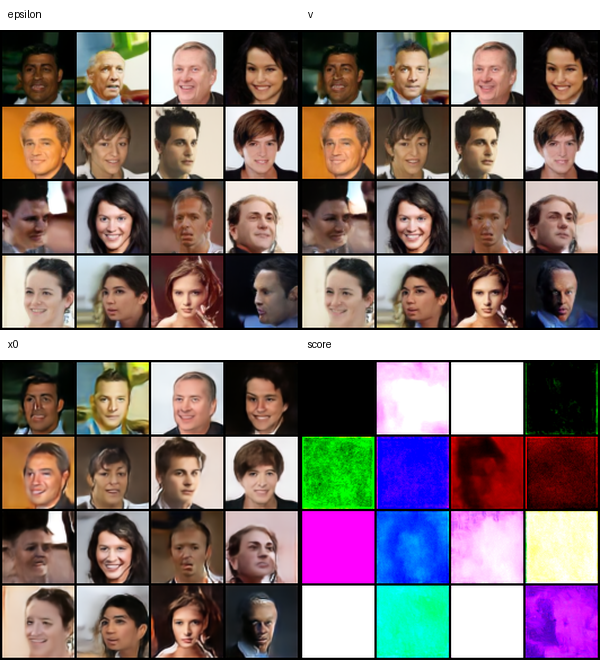
\includegraphics[width=0.95\linewidth]{figures/part4_q6_final_samples.png}
\end{center}

The original \(\epsilon\)-prediction model achieved the best KID in this run.
Among the alternatives, velocity prediction was the strongest: its KID was
close to the \(\epsilon\) baseline and the generated samples were still
face-like. Direct \(x_0\)-prediction was noticeably worse by KID, and the score
parameterization was much worse, even though it is mathematically convertible
back to a noise prediction.
}
\includeanswer{q6b}

\subq{c}{3} Compare the performance of your new parametrization with that of the original parametrization. Share your findings below.

\answerbox{}{
The main finding is that changing the prediction target changes the practical
optimization problem, even when all targets can be converted back into
\(\hat{\epsilon}_\theta\) for the same reverse sampler. In this experiment,
\(\epsilon\)-prediction remained the best overall choice with KID
\(0.006382 \pm 0.001630\). Velocity prediction was competitive with KID
\(0.008808 \pm 0.002058\), which supports the interpretation that \(v\) is a
well-conditioned coordinate system for the same \(x_0\)-\(\epsilon\)
relationship. It was not better than \(\epsilon\) here, but it was close enough
that I would consider it a reasonable alternative.

Direct \(x_0\)-prediction performed substantially worse, with KID
\(0.030816 \pm 0.003517\). Its final \(x_0\) MSE was low because that is the
direct training target, but its comparable noise MSE was worse than the
\(\epsilon\) and \(v\) models. This matters because the reverse DDPM step still
needs an accurate equivalent \(\hat{\epsilon}_\theta\). The score model had the
worst KID, \(0.254980 \pm 0.009081\), suggesting that the score target scaling
was much harder for this simple homework setup.

\begin{center}
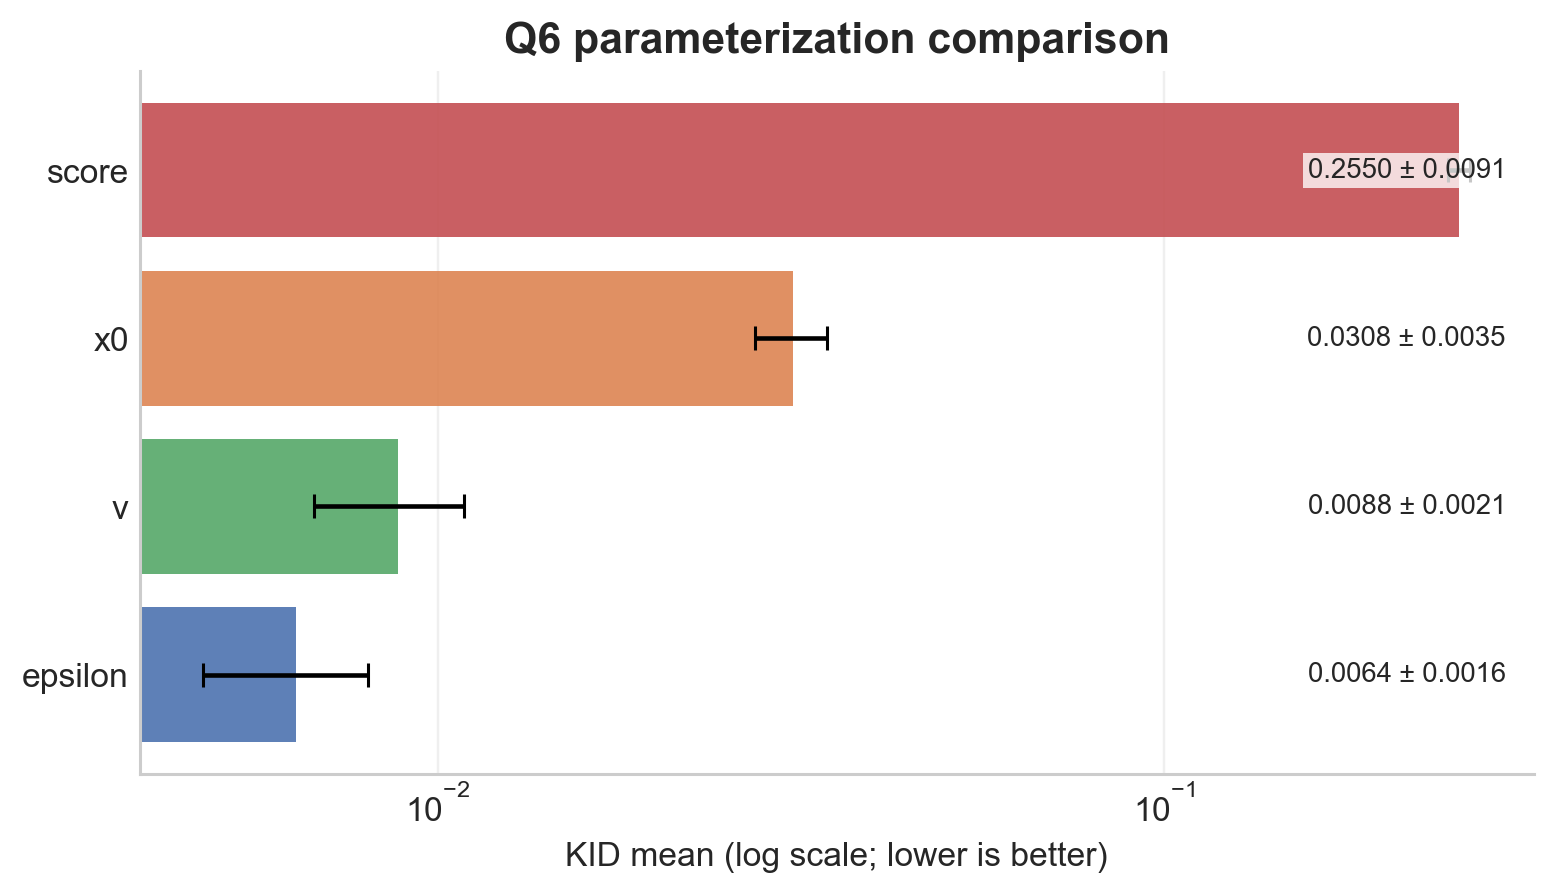
\includegraphics[width=0.78\linewidth]{figures/part4_q6_kid_bar.png}
\end{center}

\begin{center}
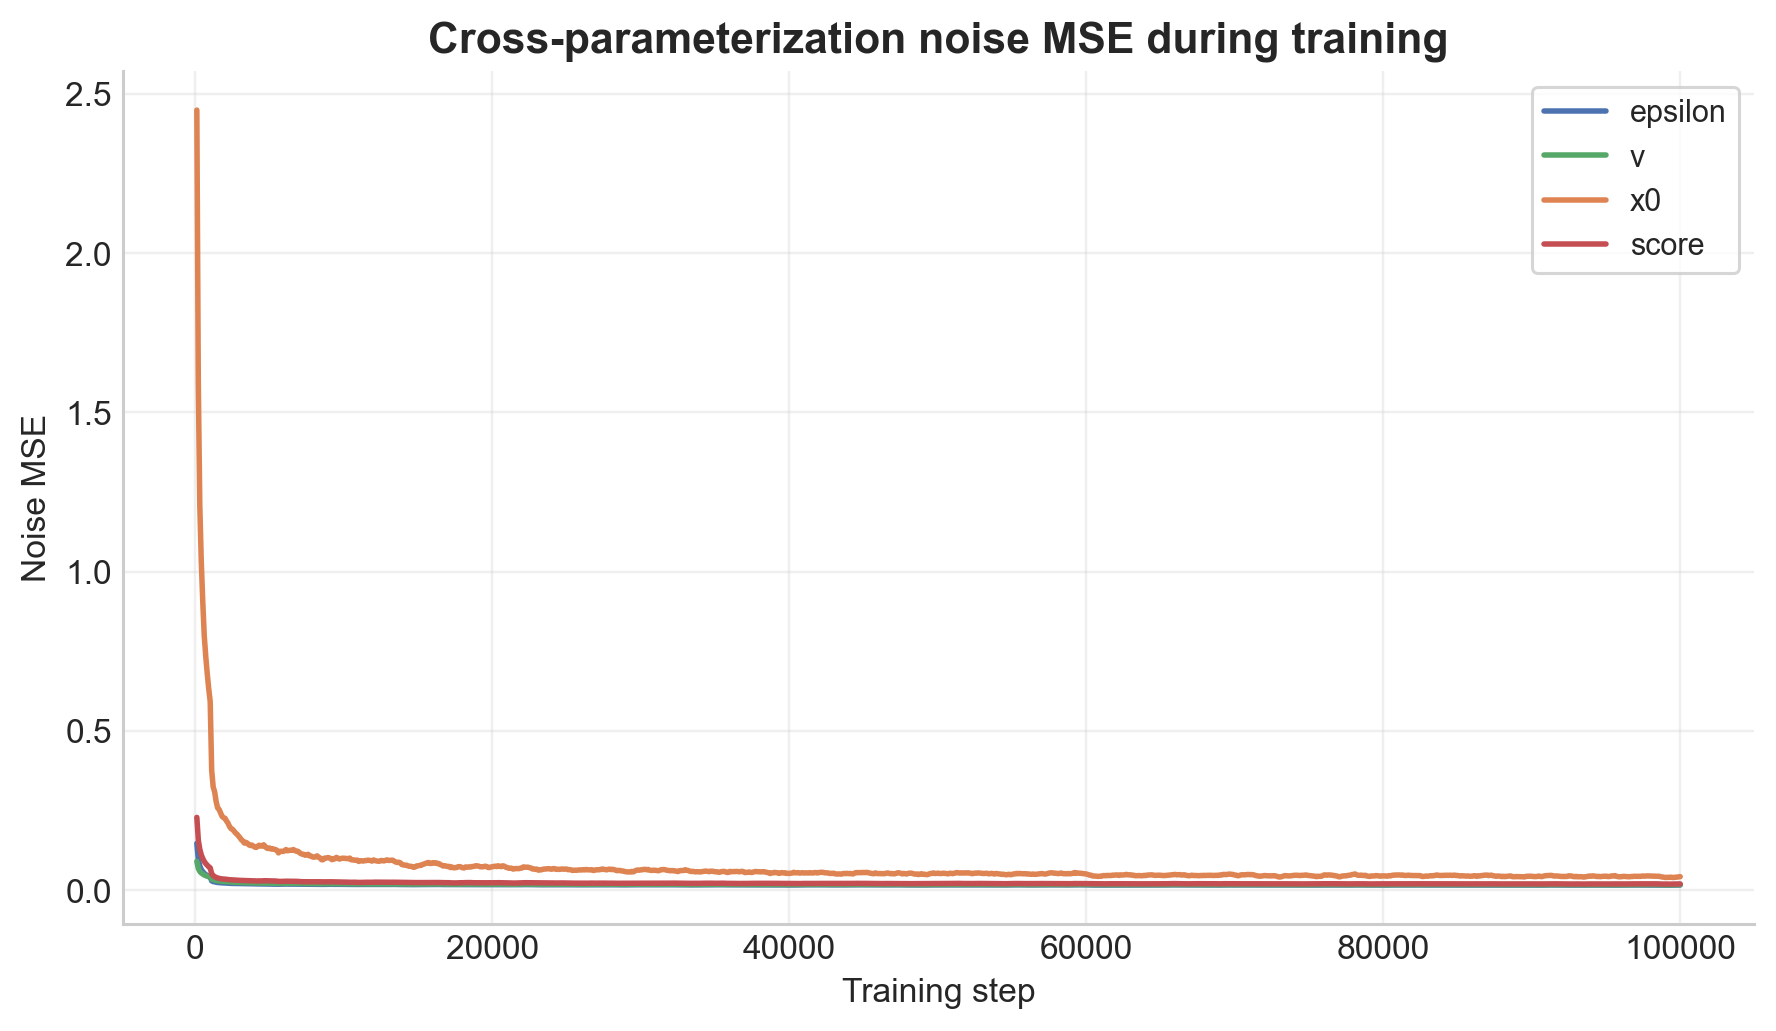
\includegraphics[width=0.78\linewidth]{figures/part4_noise_mse_curves.png}
\end{center}

\begin{center}
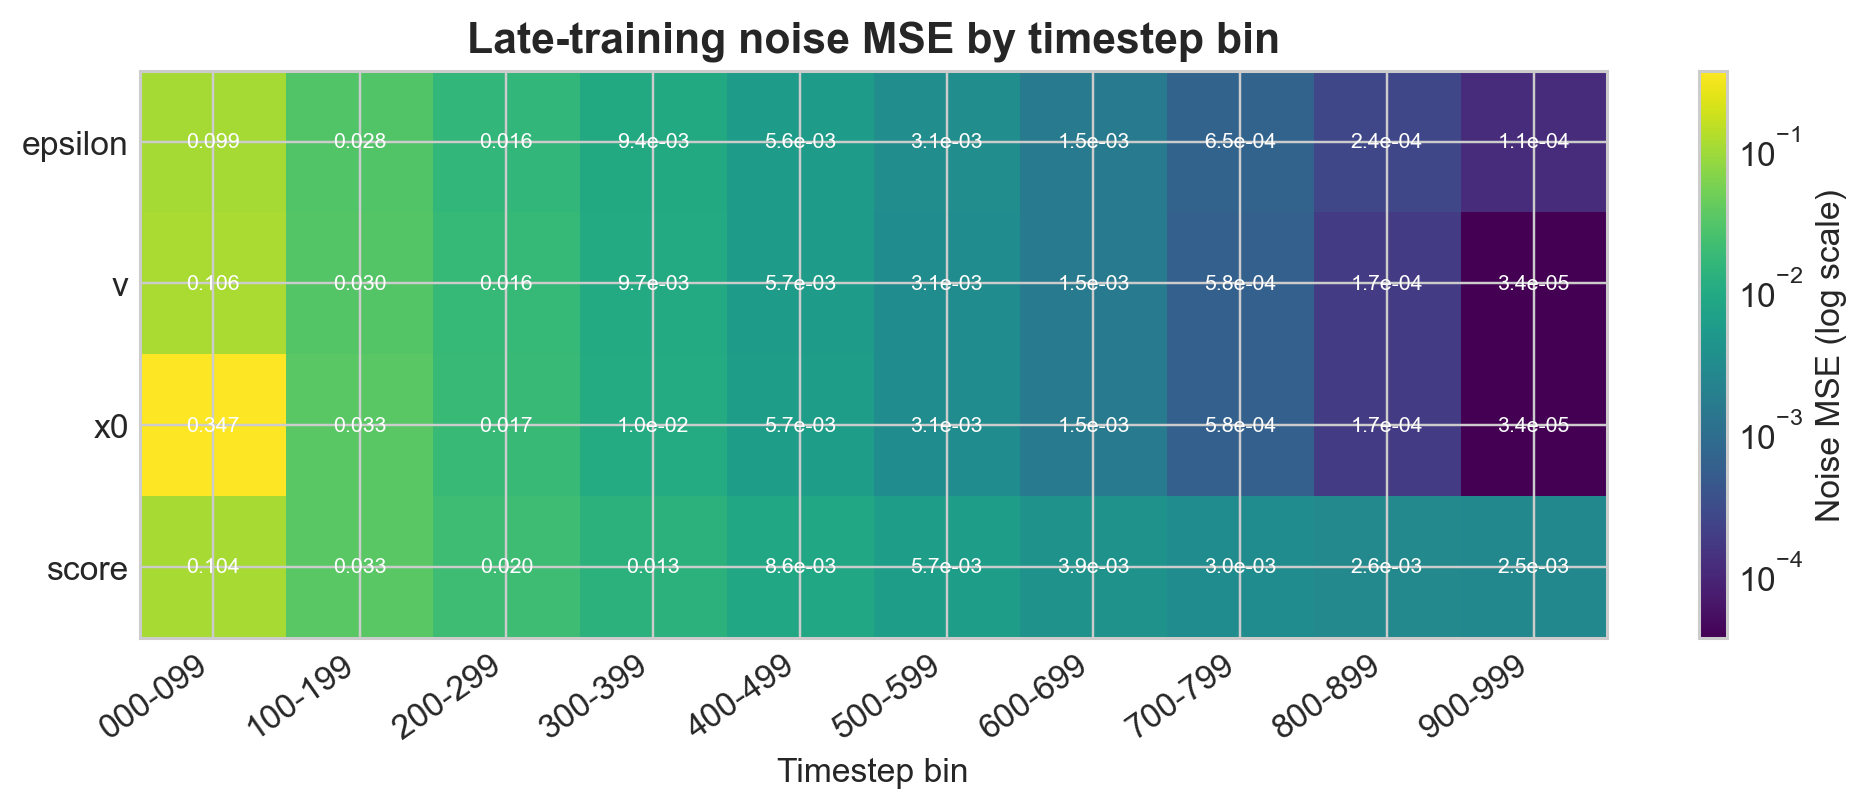
\includegraphics[width=0.78\linewidth]{figures/part4_timestep_bin_heatmap.png}
\end{center}

One useful lesson from this ablation is that raw training loss should not be
compared directly across parameterizations. Each model is minimizing a different
target scale. Comparable quantities such as KID, converted noise MSE,
qualitative samples, and timestep-bin noise MSE give a fairer picture of which
parameterization actually supports the reverse generation process.
}
\includeanswer{q6c}

\question{Sampling Steps Ablation}{10}

\subq{a}{10} DDPM typically uses 1000 timesteps for sampling, which is slow. How about using fewer steps? Report the KID scores for DDPM sampling algorithm with $100,300,500,700,900$ steps and compare with your original sampling with $1000$ steps. Include 1 sample for each number of steps to qualitatively show your comparisons as well.

\answerbox{}{
The sampler supports both the original full 1000-step stochastic DDPM reverse
chain and a deterministic strided sampler for fewer steps. For \(N<1000\), the
sampler selects \(N\) descending timesteps from \(999\) to \(0\). At each
selected timestep it predicts \(\hat{\epsilon}_\theta\), reconstructs
\[
\hat{x}_0
=
\frac{x_t-\sqrt{1-\bar{\alpha}_t}\hat{\epsilon}_\theta}
{\sqrt{\bar{\alpha}_t}},
\]
and jumps to the next selected timestep \(s\) with
\[
x_s
=
\sqrt{\bar{\alpha}_s}\hat{x}_0
+
\sqrt{1-\bar{\alpha}_s}\hat{\epsilon}_\theta.
\]
Thus, the fewer-step sampler is a deterministic strided DDIM-style sampler using
the DDPM-trained predictor, rather than the original adjacent-step posterior
applied 1000 times.

\begin{center}
\begin{tabular}{ccc}
\toprule
Sampling steps & KID mean & KID std \\
\midrule
100 & 0.013443 & 0.002852 \\
300 & 0.011125 & 0.002740 \\
500 & 0.010008 & 0.002220 \\
700 & 0.011100 & 0.003647 \\
900 & 0.010877 & 0.003623 \\
1000 & 0.006382 & 0.001630 \\
\bottomrule
\end{tabular}
\end{center}

\begin{center}
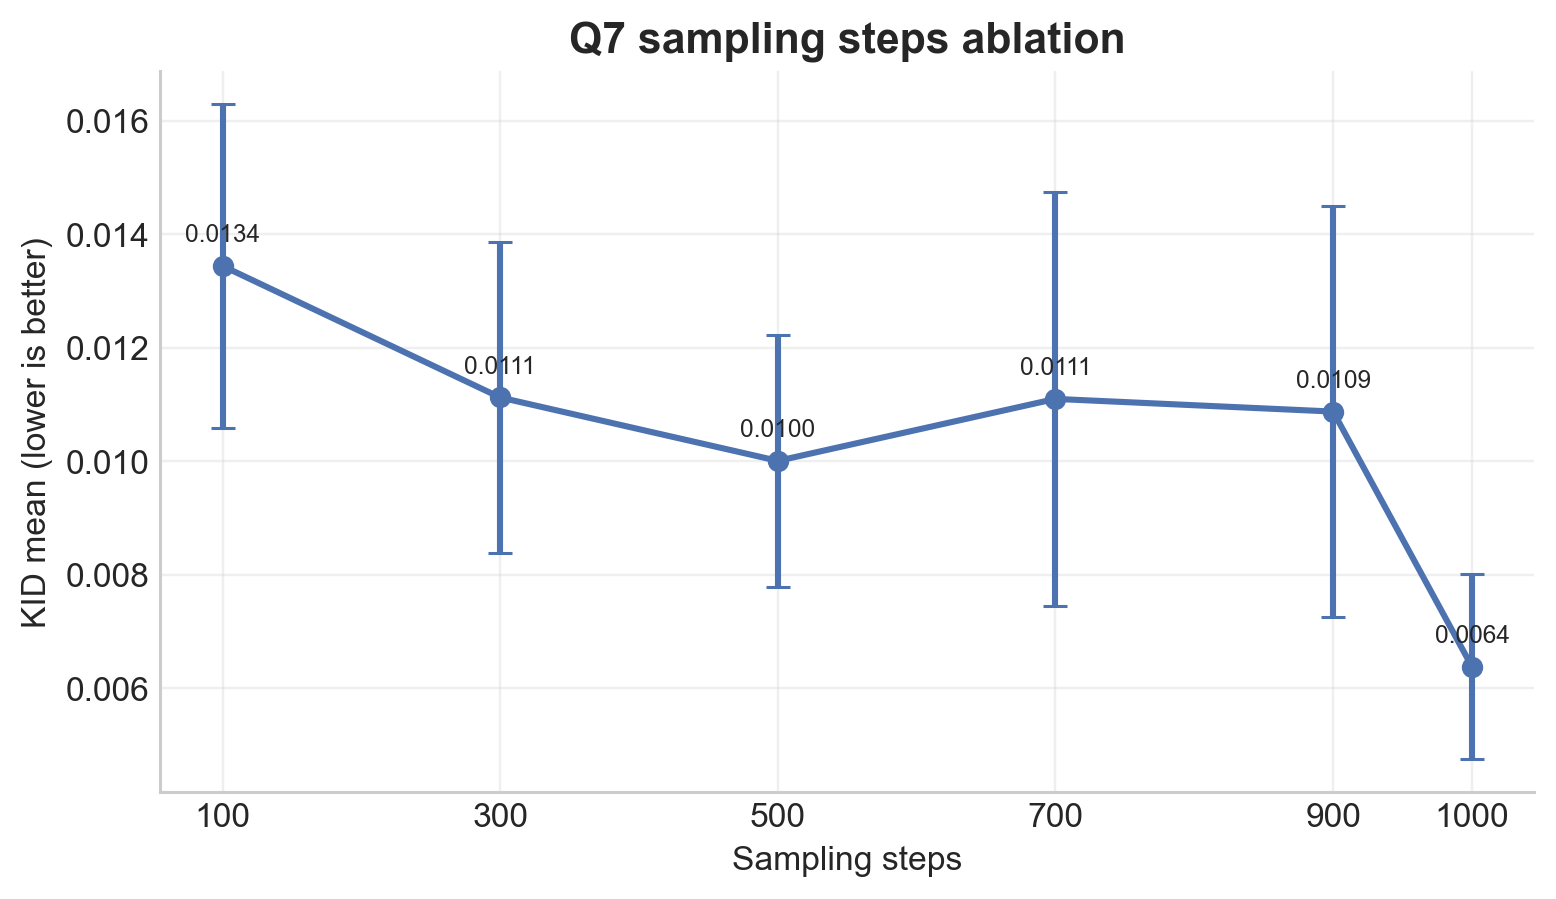
\includegraphics[width=0.78\linewidth]{figures/part4_q7_kid_vs_steps.png}
\end{center}

\begin{center}
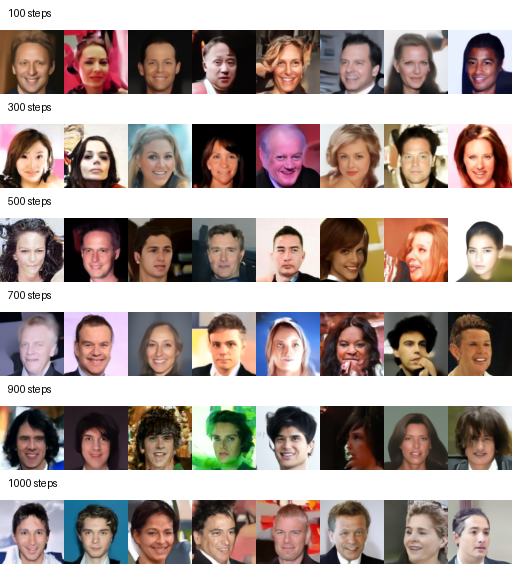
\includegraphics[width=0.95\linewidth]{figures/part4_q7_step_samples.png}
\end{center}

The full 1000-step sampler was still best, with KID
\(0.006382 \pm 0.001630\). Among the reduced-step samplers, 500 steps gave the
best KID, \(0.010008 \pm 0.002220\). The trend is not perfectly monotonic:
700 and 900 steps were slightly worse than 500 steps in this run. This can
happen because KID is estimated from a finite sample set and because changing
the stride changes the effective deterministic trajectory, not just the amount
of computation.

The sample panel shows representative generated images from each sampling-step
setting. I use it only as a qualitative sanity check, because the evaluation
script resets the random seed for each step count. That makes the generated
directories comparable and reproducible for KID, but it also means that images
with the same file index across different step counts often come from the same
initial noise sample. The more reliable comparison is therefore the KID table
and curve above. Qualitatively, the reduced-step samples remain face-like, so
the strided sampler does not completely break generation. However, the KID gap
shows the tradeoff: fewer steps make sampling faster, but the original model was
trained for the 1000-step DDPM process and still benefits from using the denser
reverse chain.
}
\includeanswer{q7a}
